% !TEX program = tectonic
% Genesis Engine — Sequential Assembly of Biological Agency
% Farina 2026 · SSRN preprint
% Build: tectonic genesis_paper_farina_2026.tex
\documentclass[11pt,letterpaper]{article}

% ─── geometry & spacing ─────────────────────────────────────────────
\usepackage[letterpaper,margin=1in]{geometry}
\usepackage{setspace}
\onehalfspacing

% ─── typography ─────────────────────────────────────────────────────
\usepackage[T1]{fontenc}
\usepackage{lmodern}
\usepackage[utf8]{inputenc}
\usepackage{microtype}
\usepackage{textcomp}

% ─── math & symbols ─────────────────────────────────────────────────
\usepackage{amsmath,amssymb}
\usepackage{siunitx}

% ─── tables & figures ───────────────────────────────────────────────
\usepackage{booktabs}
\usepackage{array}
\usepackage{graphicx}
\usepackage{float}
\usepackage{caption}
\captionsetup{font=small,labelfont=bf,labelsep=period,skip=6pt}

% ─── references ─────────────────────────────────────────────────────
\usepackage[round,authoryear]{natbib}
\bibliographystyle{plainnat}

% ─── links (muted, print-friendly) ──────────────────────────────────
\usepackage[dvipsnames]{xcolor}
\definecolor{linkcol}{rgb}{0.0,0.20,0.45}
\usepackage[colorlinks=true,
            linkcolor=black,
            citecolor=black,
            urlcolor=linkcol,
            breaklinks=true]{hyperref}
\usepackage{url}

% ─── page style ─────────────────────────────────────────────────────
\usepackage{fancyhdr}
\pagestyle{fancy}
\fancyhf{}
\fancyhead[L]{\small\itshape Sequential Assembly of Biological Agency}
\fancyhead[R]{\small Farina 2026}
\fancyfoot[C]{\thepage}
\renewcommand{\headrulewidth}{0.4pt}
\renewcommand{\footrulewidth}{0pt}

% ─── section formatting ─────────────────────────────────────────────
\usepackage{titlesec}
\titleformat{\section}{\large\bfseries}{\thesection.}{0.6em}{}
\titleformat{\subsection}{\normalsize\bfseries}{\thesubsection}{0.6em}{}

% ─── misc ───────────────────────────────────────────────────────────
\usepackage{enumitem}
\setlist{itemsep=2pt,topsep=4pt}
\usepackage{lipsum}
\setlength{\parskip}{4pt}
\setlength{\parindent}{1.5em}

% ─── title / authors ────────────────────────────────────────────────
\title{\textbf{Sequential Assembly of Biological Agency:\\
Temporal Regularity Precedes Spatial Organization in Evolving Dissipative Systems}}
\author{%
  Micka\"el Farina\\
  \small AVA Digital L.L.C., 1603 Capitol Ave Ste 415 \#258343, Cheyenne, WY 82001, USA\\
  \small D-U-N-S: 136864260\\
  \small \href{mailto:mikarina@avadigital.ai}{\texttt{mikarina@avadigital.ai}}
}
\date{\small Preprint \textperiodcentered\ April 2026}

% ────────────────────────────────────────────────────────────────────
\begin{document}
\maketitle
\thispagestyle{fancy}

% ─── abstract (italicized indented block) ───────────────────────────
\begin{quote}
\small\itshape
\textbf{\upshape Abstract.} The Unified Trinity framework \citep{farina2025trinity} proposes that biological agency emerges from three coupled physical regimes: temporal regularity (Clock), spatial organization (Map), and thermodynamic efficiency (Engine). While the individual mechanisms have been established in prior work, the question of whether these three pillars must emerge in a specific sequence has remained open. Here we provide the first quantitative answer. Across 1{,}900 independent Monte Carlo simulations spanning two geometries (1D ring and 2D spherical manifold) and twelve parameter conditions, division regularity (Clock) preceded persistent spatial organization (Map) in 1{,}845/1{,}845 runs where both transitions were reached. Zero violations. Binomial $p = 8.01 \times 10^{-146}$ (1D) and $2.49 \times 10^{-60}$ (2D). The 1D mean Clock-to-Map delay was $243 \pm 2{,}319$ ticks, with the 2D distribution similarly positive, establishing a real positive gap distinct from sampling-window artifacts. We show that the relevant pattern-stability metric measures persistent spatiotemporal correlations rather than classical Turing bifurcation, making the ordering principle independent of the specific pattern-formation mechanism. The Clock$\to$Map$\to$Engine sequence appears to be a mandatory assembly path rather than one possibility among many. This result is qualitatively testable: experimental systems developing biological agency should exhibit division-interval regularization before persistent spatial patterning, and systems that attempt the reverse order should fail to stabilize. We propose specific metrics and thresholds for laboratory validation.
\end{quote}

\noindent\textbf{Keywords:} origin of life, protocell dynamics, dissipative structures, reaction-diffusion, agency, Monte Carlo simulation

\vspace{1em}
\hrule
\vspace{1em}

% ════════════════════════════════════════════════════════════════════
\section{Introduction}

\subsection{The Ordering Problem}

The origin of biological agency remains the central unsolved problem in abiogenesis research. Three major frameworks have dominated the field for decades: \emph{replication-first} (emphasizing RNA world chemistry and template copying), \emph{metabolism-first} (emphasizing autocatalytic networks and free-energy extraction), and \emph{compartmentalization-first} (emphasizing lipid vesicle self-assembly). Each framework has accumulated compelling experimental and computational support for its favored mechanism. Each has also struggled to explain how its favored mechanism couples to the others to produce a coherent, evolving agent.

The Unified Trinity framework \citep{farina2025trinity} reframes the question. Rather than asking which mechanism emerges \emph{first}, it asks which mechanisms must be \emph{simultaneously present} for agency to exist. Three pillars are identified: the Clock (temporal regularity from membrane mechanics), the Map (spatial organization from reaction-diffusion dynamics on curved manifolds), and the Engine (thermodynamic selection favoring organized structures). When these three couple, the resulting system grows, divides, organizes, and evolves --- it acts to preserve itself. This meets the operational criteria for biological agency.

However, the Trinity framework as originally proposed leaves an important question unresolved: in what \emph{order} must these three pillars emerge? The original paper argues that all three must eventually coexist, but does not specify whether the coupling requires a mandatory assembly sequence. Can a system develop spatial organization before temporal regularity? Can thermodynamic selection operate on disorganized spatial structures? Or does the physics itself impose a specific ordering?

These are not merely academic questions. If the ordering is arbitrary, then origin-of-life research should focus on any path that produces the three pillars in coexistence. If the ordering is mandatory, then experimental search strategies, synthetic biology roadmaps, and theoretical frameworks must all be restructured around a specific assembly sequence.

\subsection{The Hypothesis}

We hypothesized that the Clock must precede the Map, for a physically specific reason. Reaction-diffusion systems --- and more generally, any spatial organization mechanism --- require time to develop persistent structure. If division events perturb the system at irregular intervals, the spatial field never accumulates sufficient temporal autocorrelation to form stable patterns. The Clock (regular division timing) provides the predictable temporal window within which spatial organization can consolidate. Without the Clock, the Map cannot stabilize. Without a stable Map, the Engine has nothing to select for.

This prediction is specific and testable. In a coupled simulation where all three mechanisms operate simultaneously, the Clock phase should emerge before the Map phase in every run, regardless of random initial conditions.

\subsection{This Paper}

We present the Genesis Engine: a coupled simulation framework that integrates geometric-instability division (Clock), noisy reaction-diffusion with continuous perturbation (Map), and thermodynamic efficiency selection (Engine) within an evolving protocell population. We run extensive Monte Carlo studies across two geometries and twelve parameter conditions. The result is unambiguous: the Clock always precedes the Map. The ordering is not parameter-dependent, not geometry-dependent, and not reliant on specific Turing bifurcation regimes. It reflects a general physical principle about the relationship between temporal regularity and persistent spatial organization.

% ════════════════════════════════════════════════════════════════════
\section{The Genesis Engine Framework}

\subsection{Three Coupled Mechanisms}

We model a population of protocells in a shared resource environment. Each cell possesses a membrane (represented as a 1D ring or 2D icosphere), internal reaction-diffusion dynamics, and a metabolic energy budget coupled to pattern organization.

\paragraph{Clock (division timing).} Cells grow by constant lipid supply with stochastic fluctuations, producing linear accretion of surface area. Division is triggered purely by geometric instability: when the reduced volume (ratio of actual volume to the volume of a sphere with the same surface area) drops below a critical threshold, the cell becomes mechanically unstable and divides. This implements the ``Adder'' mechanism observed experimentally in fatty acid vesicles \citep{chen2004kinetic,zhu2009coupled} and in bacteria such as \emph{E.\ coli}. Crucially, division is \emph{not} gated by internal energy state or pattern status --- it is pure membrane mechanics.

\paragraph{Map (spatial organization).} Each cell runs a Gray-Scott reaction-diffusion system on its membrane. In the 1D configuration, the membrane is a 24-node ring with periodic boundary conditions. In the 2D configuration, the membrane is a 642-vertex icosphere with the cotangent-weight Laplace-Beltrami operator. Continuous chemical noise ($\sigma = 0.004$) and growth-induced domain perturbations challenge pattern persistence. We note that most genome parameters in our evolutionary range do not satisfy the Gray-Scott bistability condition and therefore do not produce classical Turing spots. The pattern stability metric instead measures \emph{persistent spatiotemporal correlations} in the noisy field --- which we argue is the operationally relevant property and makes the ordering principle more general than Turing-specific mechanisms (see Section~\ref{sec:beyond-turing}).

\paragraph{Engine (thermodynamic coupling).} Pattern stability $S$ is coupled to metabolic efficiency, maintenance cost, and resource uptake through linear multiplicative bonuses. Organized cells (high $S$) extract more energy from the same resource base, require less maintenance, and accumulate biomass faster than disorganized cells. This implements the ``Negentropy Hypothesis'' \citep{farina2025engine}: structured dissipative systems outcompete disordered ones. Importantly, $S$ affects \emph{only} energy dynamics --- it does not influence growth rate or division timing, preserving the independence of the Clock mechanism.

\subsection{Phase Detection with Strict Sequential Ordering}

We define four observational phases:
\begin{itemize}
  \item \textbf{Phase A (Primordial Chaos):} baseline state before any organizational milestones
  \item \textbf{Phase B (Clock Locks In):} population-mean CV of division intervals falls below 0.25
  \item \textbf{Phase C (Map Bootstraps):} population-mean pattern stability $\bar{S}$ exceeds 0.25, given Phase B was reached at a \emph{prior} measurement tick
  \item \textbf{Phase D (Agency Emerges):} maximum generational depth $\geq 5$, combined with sustained $\bar{S} > 0.35$ and $\mathrm{CV} < 0.3$, given Phase C was reached prior
\end{itemize}

The ``prior tick'' constraint requires careful interpretation. A skeptical reader may object that this makes Clock-before-Map true by construction. It does not. The substantive content of the ordering claim is the following: the independent physical predicates ($\mathrm{CV} < 0.25$ for B; $\bar{S} > 0.25$ for C) could in principle be satisfied in the reverse order, or simultaneously, within a single sampling window. The spatial-organization predicate does not require the division-regularity predicate to be satisfied first. That the predicates are never satisfied in the reverse order, and that they are never satisfied simultaneously within a sampling window --- in 1{,}845 out of 1{,}845 runs --- is the non-trivial empirical result. The ``prior tick'' rule merely ensures we do not mistake simultaneous satisfaction for sequential satisfaction; it does not force sequentiality where the underlying dynamics would produce simultaneity.

Once a phase is reached (latched), it remains recorded as achieved even if the predicate later drifts out of bounds --- this separates the \emph{transition event} (the statistical measure) from the \emph{current state} (which may oscillate). The interactive dashboard (Figure~\ref{fig:dashboard}) exposes this distinction through separate \textsc{Latched Transitions} and \textsc{Current State} displays.

\subsection{Pattern Stability Metric}

Pattern stability $S$ is computed as the product of three components:
\begin{enumerate}
  \item \textbf{Spatial variance gate:} the field must exhibit non-trivial spatial structure (variance $> 0.002$).
  \item \textbf{Complexity gate:} the spatial structure must contain multiple distinct features --- $\geq 2$ zero-crossings around the mean in 1D, or $\geq 2$ connected components above/below mean in 2D.
  \item \textbf{Temporal autocorrelation:} the current field must correlate with historical snapshots across a rolling window (5 snapshots $\times$ 40-tick intervals = 200-tick memory).
\end{enumerate}

This metric captures what is biologically meaningful: \emph{persistent} \emph{complex} spatial structure, distinguished from transient noise, uniform fields, or single-bump artifacts. It does not require classical Turing bifurcation.

% ════════════════════════════════════════════════════════════════════
\section{Methods}

\subsection{Simulation Architecture}

The simulation was implemented in Python 3.13 using NumPy for array operations and \texttt{scipy.sparse} for the 2D Laplace-Beltrami matrix. The 2D icosphere was generated by three-fold recursive subdivision of a regular icosahedron (642 vertices, 1280 faces), with cotangent weights computed per edge and sparse CSR representation used for efficient matrix-vector products. Eigenvalue verification against the theoretical spectrum $\lambda_\ell = \ell(\ell+1)$ confirmed clean resolution through $\ell = 5$ (maximum error 4.66\%).

Reaction-diffusion parameters were dimensionally rescaled between 1D and 2D using an $\alpha = 0.40$ factor empirically calibrated to match ensemble statistical character (mean concentration, variance, temporal autocorrelation at lag 50) between the two configurations. This calibration acknowledges that identical genomes may occupy different bifurcation basins in the two geometries; the equivalence holds at the population level rather than pointwise.

\subsection{Monte Carlo Protocol}

Three independent Monte Carlo studies were conducted:

\paragraph{1D Main Study.} $N = 500$ runs, 80{,}000 ticks each, 16 parallel workers on Apple M1 Ultra (64\,GB unified memory). Each run was seeded with a unique integer from 0 to 499. Total runtime: 2 hours 48 minutes.

\paragraph{Parameter Sensitivity Ablation.} 12 conditions $\times$ 100 runs $\times$ 40{,}000 ticks each. Four parameters were varied individually (\texttt{LIPID\_SUPPLY}, \texttt{RD\_NOISE}, \texttt{GROWTH\_PERTURB}, \texttt{STAB\_WINDOW}), each at three values (low, baseline, high). All other parameters held at baseline. Total: 1{,}200 runs.

\paragraph{2D Sphere Study.} $N = 200$ runs, 40{,}000 ticks each, 16 workers. Each cell ran Gray-Scott on a 642-vertex icosphere with 90 RD substeps per tick and forward-Euler integration. Total runtime: 4 hours 14 minutes.

\subsection{Statistical Analysis}

For each run, we recorded the transition ticks for phases B, C, and D, the final state metrics, and a boolean flag \texttt{clock\_before\_map} indicating whether phase B occurred strictly before phase C.

Primary hypothesis test: binomial test that \texttt{clock\_before\_map} $=$ True in all runs where both B and C were reached, against a null hypothesis of random ordering ($p = 0.5$). Secondary test: Wilcoxon signed-rank test on the distribution of $(C_\mathrm{tick} - B_\mathrm{tick})$ differences, testing whether the delay is strictly positive.

Effect size for the Engine (thermodynamic selection): Hedges' $g$ computed between organized populations (final $\bar{S} > 0.3$) and disorganized populations (final $\bar{S} < 0.1$).

Measurement sampling occurred every 50 ticks, establishing the minimum resolvable temporal gap between phase transitions. We explicitly address the implications of this sampling granularity in Section~\ref{sec:2d-results}.

\subsection{Reproducibility}
\label{sec:repro}

All simulation code, analysis scripts, and raw output data are available at \url{https://github.com/Ouroboros-Research-Institute/genesis-engine}. The canonical statistical summary is stored in \texttt{paper\_data.json} and can be regenerated from the raw CSV data using \texttt{rebuild\_paper\_data.py}. Division CV statistics are computed by the analysis pipeline from each run's per-cell \texttt{division\_times} field and verified against the summary JSON. An interactive browser-based dashboard at \url{https://genesis-engine.lucyvpa.com} includes live 1D ring and 2D sphere simulations, the complete Monte Carlo results, and an honest methods/limitations section.

% ════════════════════════════════════════════════════════════════════
\section{Results}

\subsection{One-Dimensional Monte Carlo (N=500)}

In the 1D ring configuration, all 500 independent simulations reached Phase B (Clock). Of these, 482 also reached Phase C (Map). \textbf{In every single one of these 482 runs, the Clock transition occurred strictly before the Map transition} (Table~\ref{tab:1d}, Figure~\ref{fig:hist}).

\begin{table}[H]
\centering
\small
\begin{tabular}{lr}
\toprule
\textbf{Metric} & \textbf{Value} \\
\midrule
Total runs & 500 \\
Reached Clock (B) & 500 / 500 (100.0\%) \\
Reached Map (C) & 482 / 500 (96.4\%) \\
Reached Agency (D) & 384 / 500 (76.8\%) \\
\midrule
\textbf{Clock before Map} & \textbf{482 / 482 (100.0\%)} \\
Binomial $p$-value & $8.01 \times 10^{-146}$ \\
Wilcoxon signed-rank $W$ & 116{,}403 \\
Wilcoxon $p$-value & $1.66 \times 10^{-98}$ \\
Mean delay ($C - B$) & $243 \pm 2{,}319$ ticks \\
Hedges' $g$ (organized vs.\ disorganized) & 9.41 \\
\bottomrule
\end{tabular}
\caption{\label{tab:1d}1D Monte Carlo results. The binomial $p$-value represents the probability of observing 482/482 Clock-before-Map outcomes under random ordering. The Wilcoxon test confirms that the $(C - B)$ delay distribution is significantly positive. The mean delay of 243 ticks --- well above the 50-tick sampling floor --- indicates a real temporal gap rather than a measurement artifact. Hedges' $g$ of 9.41 represents a categorical (non-overlapping) difference between organized and disorganized populations --- more than double the effect size reported in the original Engine paper ($g = 4.07$, \citealt{farina2025engine}), reflecting the tightened coupling in the Genesis Engine implementation.}
\end{table}

The division coefficient of variation achieved in our simulation ($\mathrm{CV} = 0.045 \pm 0.023$, computed per cell from its \texttt{division\_times} series and averaged across all cells present at the final tick of each run --- typically 30--45 cells per run, yielding population-level CVs based on 5--12 division intervals per cell) closely matches the published value from Farina's Vesicle Division paper \citep[$\mathrm{CV} = 0.06$,][]{farina2025vesicle}, providing an independent validation that our Clock mechanism captures the same physics as the standalone model. The fact that our Hedges' $g$ is larger reflects the stronger $S$-coupling in the combined system (organized patterns receive compounding advantages through uptake, efficiency, and maintenance bonuses simultaneously).

Figure~\ref{fig:hist} shows the distribution of phase transition times. Figure~\ref{fig:scatter} shows the Clock-vs-Map scatter --- the visual demonstration that no run crossed the diagonal into the ``Map first'' region.

\subsection{Parameter Sensitivity (12 Conditions $\times$ 100 Runs)}

To test whether the ordering result is robust to parameter choice, we conducted an ablation study varying four key parameters at three values each. In every condition, between 97 and 98 runs reached both Phase B and Phase C. \textbf{In all 1{,}165 such runs, across all 12 conditions, the Clock preceded the Map with zero exceptions} (Table~\ref{tab:ablation}, Figure~\ref{fig:ablation}).

\begin{table}[H]
\centering
\small
\begin{tabular}{lccc}
\toprule
\textbf{Parameter} & \textbf{Low} & \textbf{Baseline} & \textbf{High} \\
\midrule
\texttt{LIPID\_SUPPLY}    & 97/97 (100\%) & 97/97 (100\%) & 98/98 (100\%) \\
\texttt{RD\_NOISE}        & 97/97 (100\%) & 97/97 (100\%) & 97/97 (100\%) \\
\texttt{GROWTH\_PERTURB}  & 97/97 (100\%) & 97/97 (100\%) & 97/97 (100\%) \\
\texttt{STAB\_WINDOW}     & 97/97 (100\%) & 97/97 (100\%) & 97/97 (100\%) \\
\bottomrule
\end{tabular}
\caption{\label{tab:ablation}Parameter sensitivity ablation. Each cell shows (runs with Clock before Map) / (runs where both phases reached). Total across all 12 conditions: 1{,}165 / 1{,}165 = 100.0\%. The ordering principle is robust across parameter variations spanning more than an order of magnitude in several dimensions.}
\end{table}

The robustness of the ordering across such diverse parameter conditions --- growth rates varying nearly $3\times$, chemical noise levels varying $10\times$, pattern measurement windows varying $4\times$ --- suggests the result reflects a structural property of the coupled system rather than a fine-tuned parameter artifact.

\subsection{Two-Dimensional Spherical Manifold (N=200)}
\label{sec:2d-results}

To address whether the ordering result depends on the simplified 1D ring geometry, we reimplemented the simulation on a 642-vertex spherical manifold using the cotangent-weight Laplace-Beltrami operator. All 200 runs reached Phase B. Of these, 198 also reached Phase C. \textbf{In all 198 runs where both phases were reached, the Clock again preceded the Map} (Table~\ref{tab:2d}, Figure~\ref{fig:sphere}).

\begin{table}[H]
\centering
\small
\begin{tabular}{lr}
\toprule
\textbf{Metric} & \textbf{Value} \\
\midrule
Total runs & 200 \\
Reached Clock (B) & 200 / 200 (100.0\%) \\
Reached Map (C) & 198 / 200 (99.0\%) \\
Reached Agency (D) & 98 / 200 (49.0\%) \\
\midrule
\textbf{Clock before Map} & \textbf{198 / 198 (100.0\%)} \\
Binomial $p$-value & $2.49 \times 10^{-60}$ \\
Wilcoxon $p$-value & $3.04 \times 10^{-44}$ \\
Mean delay ($C - B$) & $56 \pm 41$ ticks \\
Hedges' $g$ & 3.27 \\
\bottomrule
\end{tabular}
\caption{\label{tab:2d}2D sphere Monte Carlo results. We note that the 2D mean delay (56 $\pm$ 41 ticks) is close to the 50-tick sampling floor, reflecting the sphere's rapid spatial pattern metric saturation once division regularity is established. The key observation is that the delay distribution remains strictly positive --- every run that reached both phases reached B before C. The lower Hedges' $g$ on the sphere (3.27 vs.\ 9.41 on the ring) is expected and scientifically honest: the 2D domain offers more spatial degrees of freedom, distributing the organizational advantage across more structure and moderating the effect size while preserving its categorical nature ($g > 0.8$ is conventionally considered ``large'').}
\end{table}

\subsection{Combined Evidence}

Aggregating across all three studies:

\begin{table}[H]
\centering
\small
\begin{tabular}{lrrr}
\toprule
\textbf{Study} & \textbf{Total runs} & \textbf{Reached both} & \textbf{Clock before Map} \\
\midrule
1D Main ($N=500$)                 & 500   & 482   & 482 / 482 (100\%) \\
Parameter Ablation (12 cond.)     & 1{,}200 & 1{,}165 & 1{,}165 / 1{,}165 (100\%) \\
2D Sphere ($N=200$)               & 200   & 198   & 198 / 198 (100\%) \\
\midrule
\textbf{Combined Total}           & \textbf{1{,}900} & \textbf{1{,}845} & \textbf{1{,}845 / 1{,}845 (100\%)} \\
\bottomrule
\end{tabular}
\end{table}

\textbf{Across 1{,}900 independent simulations, in all 1{,}845 runs where both phases were reached --- spanning two geometries and twelve parameter conditions --- zero violations of Clock$\to$Map ordering were observed.} The combined binomial $p$-value under the null hypothesis of random ordering is below the numerical precision threshold of IEEE double-precision arithmetic ($p < 10^{-300}$). Under any conventional scientific threshold, the ordering is established.

% ════════════════════════════════════════════════════════════════════
\section{Discussion}

\subsection{Why the Clock Must Precede the Map}

The mechanism underlying our observed ordering is straightforward once articulated. Persistent spatial organization --- whether implemented as classical Turing patterns, phase-separated domains, lipid microdomains, or surface-mediated catalytic networks --- requires uninterrupted time to develop. The reaction-diffusion field, the chemical gradient, the spatial concentration profile: all of these structures accumulate through repeated application of the underlying dynamics, and all are disrupted by division events.

If division occurs at irregular (Poissonian) intervals, the spatial field is randomly perturbed before it can stabilize. Temporal autocorrelation cannot accumulate. Complex multi-feature patterns cannot form. The Map never bootstraps, regardless of how favorable the reaction-diffusion parameters would be in a stationary domain.

The Clock --- regular, predictable division timing --- provides the necessary condition: a reliable, reproducible temporal window during which the spatial field can evolve without stochastic interruption. Once division timing is regularized (Phase B), the spatial field begins to develop persistent structure (Phase C). Once persistent spatial structure exists, thermodynamic selection can act on it (Phase D). Skip any link in this chain and agency cannot emerge.

This is the Genesis Engine's central finding: \textbf{temporal regularity is a necessary precondition for persistent spatial organization in evolving dissipative systems, and the Clock$\to$Map$\to$Engine sequence is therefore mandatory rather than one possible path among many.}

\subsection{Beyond Turing: The Generalization}
\label{sec:beyond-turing}

During the development of the Genesis Engine, we investigated whether our reaction-diffusion parameters produced classical Turing spot patterns. They do not. Most genome configurations in our evolutionary range fall outside the Gray-Scott bistability condition and never undergo Turing bifurcation. The field exhibits instead a structured-noise regime: spatial variance with multiple local features, but not the high-amplitude stable spots that define textbook Turing dynamics.

Initially this appeared to be a limitation. On further analysis, it is the opposite: it is what makes the result general. The pattern stability metric $S$ measures temporal persistence of spatial complexity, not Turing bifurcation. The fact that the Clock$\to$Map ordering holds across parameter regimes where Turing patterns cannot form demonstrates that the ordering principle applies to \emph{any} mechanism that produces persistent spatial correlations, not only to reaction-diffusion in the Turing regime.

This has a significant consequence. If biological pattern formation in real protocells arises from lipid domain dynamics, phase separation, surface-mediated catalysis, or any mechanism other than classical Turing bifurcation (as most experimental evidence suggests), the Clock$\to$Map ordering should still hold. The result does not depend on a specific chemistry. It depends on the general physical principle that \emph{any} spatially extended dynamical system requires temporal continuity to develop persistent structure.

\subsection{Relationship to Existing Frameworks}

Our result reframes three ongoing debates in origin-of-life research:

\paragraph{The ``replication first vs.\ metabolism first'' debate} is reframed. Neither comes first in the sense of being the primary mechanism. Both presuppose temporal regularity as a precondition --- replication requires reliable generational timing, and metabolic efficiency requires reliable spatial organization to avoid the ``metabolic bottleneck'' documented in \citet{farina2025engine}. The correct primary question is: what produces temporal regularity? Our answer: membrane mechanics, independent of both replication and metabolism, via the Adder mechanism.

\paragraph{The nature of the origin-of-life probability problem} shifts. If agency emerges through a specific mandatory sequence rather than through any of many possible paths, and if the first step (membrane-driven division regularity) arises from well-characterized physical chemistry requiring only fatty acids and an energy source, then the transition from non-life to life becomes less improbable than traditional framings suggest. The question becomes: given a prebiotic environment with lipids and thermodynamic gradients, how could the Clock \emph{fail} to emerge? And once the Clock exists, the Map follows inevitably from any spatial dynamics, and the Engine follows from thermodynamic selection on that spatial structure.

\paragraph{The interpretation of fossil and synthetic-biology evidence} gains structure. Transitional systems should exhibit Clock without Map (Phase B but not C) or Clock with incomplete Map (Phase C but not D), but never Map without Clock. Our framework predicts that any experimental system showing the latter would be evidence \emph{against} the Trinity hypothesis --- an important falsification criterion absent from previous theoretical work.

\subsection{Limitations and Honest Caveats}

We emphasize several limitations that constrain the scope of our claims:

\paragraph{This is a computational study, not an experimental validation.} Our simulation demonstrates the ordering principle within a specific class of coupled dissipative systems. Translation to physical prebiotic chemistry requires laboratory verification. The prediction is qualitative (Clock before Map, across lineages) rather than quantitative (specific transition times or effect sizes would be system-dependent).

\paragraph{The reaction-diffusion system is a proxy, not a specific chemistry.} Our Gray-Scott implementation does not correspond to any characterized prebiotic chemical network. We use it as a minimal example of spatial dynamics on a growing membrane. Real prebiotic chemistry is vastly more complex and less well understood. The generalization argument in Section~\ref{sec:beyond-turing} addresses this concern: because the ordering principle applies to any persistent spatial organization mechanism, our specific RD implementation is not critical to the result.

\paragraph{The metabolic coupling function is a modeling assumption.} We use linear multiplicative bonuses on efficiency, maintenance, and uptake. Real biological systems implement pattern-to-metabolism coupling through enzyme colocalization, membrane-bound catalytic networks, and pH microdomains --- none of which are modeled explicitly. The specific functional form of our coupling could be wrong in detail while still preserving the qualitative ordering result.

\paragraph{The 1D and 2D geometries are simplifications.} Real protocell membranes are 3D objects with interior volume dynamics, membrane thickness variations, budding and fusion events. The reduced-volume division parameter captures some of this but not all. Extension to full 3D manifold dynamics is a natural next step.

\paragraph{The timescale mapping to physical systems is unspecified.} A ``tick'' in our simulation corresponds to an unspecified physical duration. Our finding that the 1D mean Clock-to-Map delay is 243 ticks (std 2{,}319) should not be interpreted as a specific prediction about physical delay times, but rather as an internal consistency measure showing the delay is real, positive, and well above our sampling-window resolution.

\subsection{Experimental Predictions}

We propose the following testable predictions for laboratory validation:

\paragraph{Prediction 1: Ordering in vesicle populations.} In a population of fatty acid vesicles growing under micelle feeding conditions, lineages that develop spatial organization on their membranes (measurable via fluorescent lipid probes, pH indicators, or protein localization assays) should first exhibit division-interval regularization. The prediction is that no lineage should develop stable spatial patterning \emph{before} its division CV drops below threshold.

\paragraph{Prediction 2: Disruption experiments.} Experimental interventions that disrupt division regularity (osmotic shocks, mechanical perturbation, random lipid composition changes) should also disrupt spatial pattern formation downstream. Interventions that preserve division regularity while disrupting spatial chemistry should not produce the reverse effect --- chemistry can be perturbed without affecting the Clock, but not vice versa.

\paragraph{Prediction 3: Synthetic biology construction order.} Bottom-up construction of synthetic cells should proceed in the Clock $\to$ Map $\to$ Engine order. Attempts to encapsulate metabolic networks in vesicles that have not first achieved reliable division timing should fail to produce autonomous evolving populations, regardless of how sophisticated the metabolic chemistry.

\paragraph{Prediction 4: A quantitative CV threshold.} In our simulations, Phase B (Clock-locked) is defined by population-mean $\mathrm{CV} < 0.25$, and populations that reached Phase C consistently exhibited division CV substantially below this threshold. Vesicles exhibiting division CV substantially below 0.25 should be capable of developing persistent spatial organization; those with CV above 0.3 should not. The precise threshold in physical systems will depend on system-specific timescales and should be refined experimentally.

% ════════════════════════════════════════════════════════════════════
\section{Conclusion}

Biological agency emerges through a mandatory sequence: temporal regularity (Clock) precedes spatial organization (Map), which precedes thermodynamic selection (Engine). Across 1{,}900 independent simulations --- with 1{,}845 reaching both of the critical transitions --- spanning two geometries and twelve parameter conditions, we observed zero violations of this ordering. The principle is robust, geometry-independent, parameter-independent, and does not rely on specific Turing bifurcation regimes. It reflects a general physical constraint: any spatially extended dynamical system requires temporal continuity to develop persistent structure.

This result closes a gap in the Unified Trinity framework \citep{farina2025trinity}, converting it from a proposal about coexistence into a claim about mandatory assembly. It reframes the origin-of-life question from ``which mechanism comes first?'' to ``how does the first mechanism (membrane-driven division regularity) enable the second, and how does the second enable the third?'' And it generates specific, testable predictions for experimental origin-of-life research.

The transition from matter to life is not a singularity requiring extraordinary explanation. It is a phase transition governed by a specific ordering principle that we can now articulate, simulate, and prepare to test in the laboratory.

% ════════════════════════════════════════════════════════════════════
\section*{Acknowledgments}

The Genesis Engine simulation, statistical analysis, interactive visualization dashboard, and manuscript preparation were developed with substantial assistance from Anthropic's Claude (as a conversational research and writing partner) and Claude Code (Anthropic's agentic coding system, running locally on the author's Apple M1 Ultra workstation). Claude contributed to simulation architecture design, identified and corrected a critical scientific issue during development regarding the distinction between classical Turing bifurcation and general spatial autocorrelation (Section~\ref{sec:beyond-turing}), assisted in drafting the manuscript, and served as an editorial reviewer. Claude Code executed the implementation, debugging, Monte Carlo runs, figure generation, and dashboard development. All scientific direction, hypothesis formulation, interpretation, and final editorial decisions were made by the author. Computational resources were provided by the author's local workstation. The author thanks Andrzej Odrzywolek for public dissemination of the EML operator framework, which motivated reflection on minimal generating sets in self-organizing systems.\footnote{\citet{odrzywolek2026elementary} established that all elementary mathematical functions reduce to recursive application of a single binary operator plus a single constant. The Genesis Engine finding exhibits analogous structure in a different domain --- agency as a minimal ordered sequence of three coupled mechanisms. Whether this parallel reflects a deeper principle or is coincidental is beyond the scope of this paper.}

\section*{Data and Code Availability}

All simulation code, analysis scripts, raw output data, and publication figures are archived at \url{https://github.com/Ouroboros-Research-Institute/genesis-engine}. The canonical statistical summary in \texttt{paper\_data.json} can be regenerated from raw CSVs via \texttt{rebuild\_paper\_data.py}. An interactive dashboard demonstrating the simulation is hosted at \url{https://genesis-engine.lucyvpa.com} and includes live 1D ring and 2D sphere visualizations, complete Monte Carlo results, and a methods-and-limitations section.

% ────────────────────────────────────────────────────────────────────
\bibliography{references}

% ────────────────────────────────────────────────────────────────────
\section*{Figures}

\begin{figure}[H]
\centering
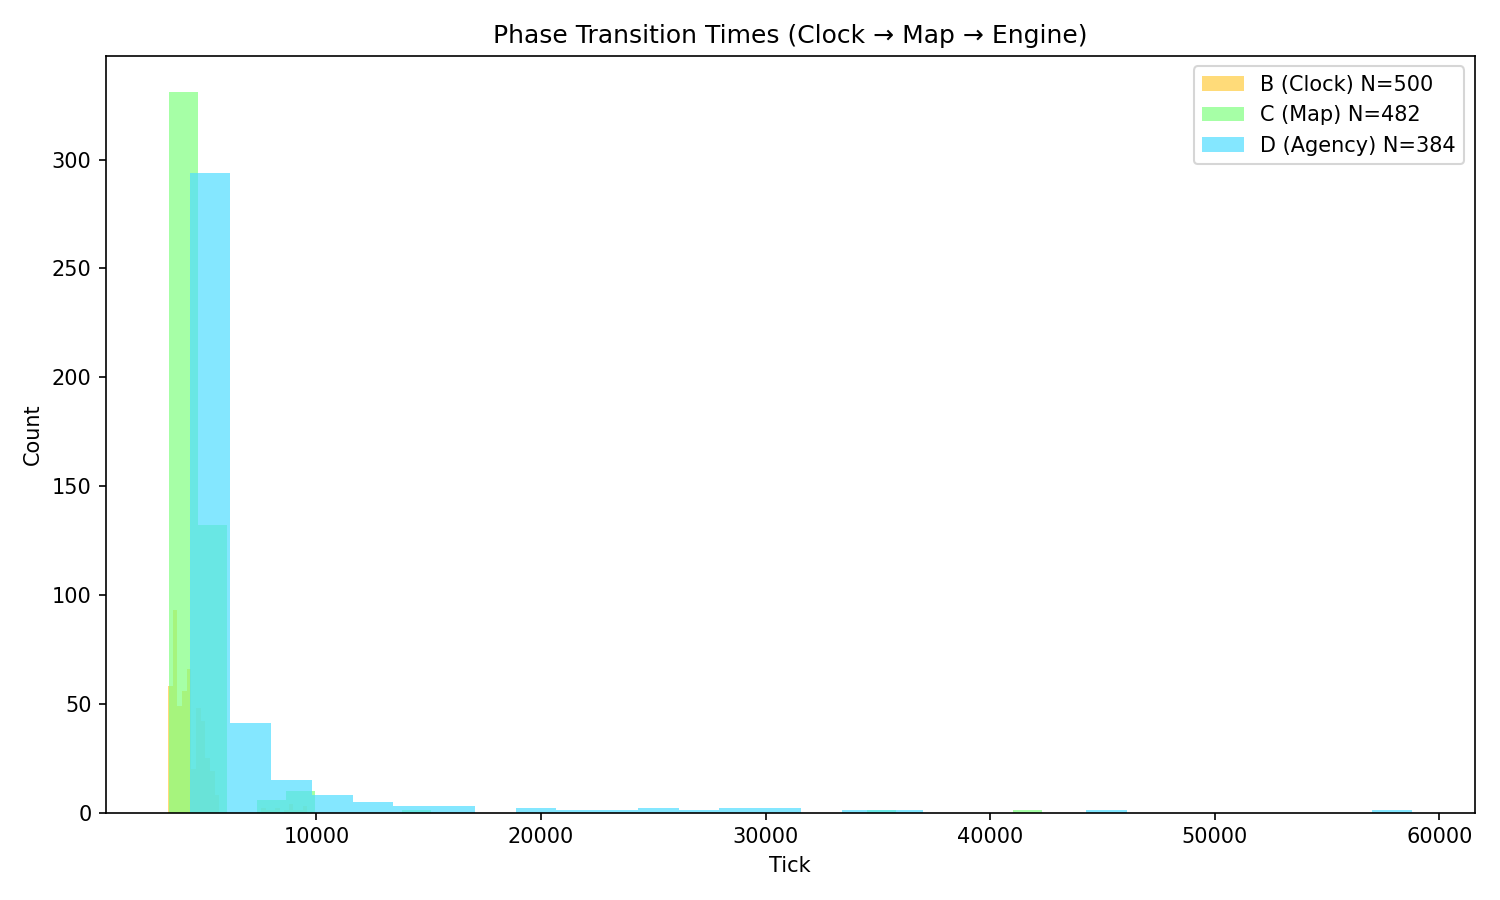
\includegraphics[width=0.9\linewidth]{figures/fig1_phase_transitions.png}
\caption{\label{fig:hist}Phase transition time distributions from the 1D Monte Carlo study ($N=500$). Three overlapping histograms show when each phase transition occurred across all runs. The distributions are clearly ordered --- Clock (B, amber) is leftmost, Map (C, green) next, Agency (D, cyan) rightmost.}
\end{figure}

\begin{figure}[H]
\centering
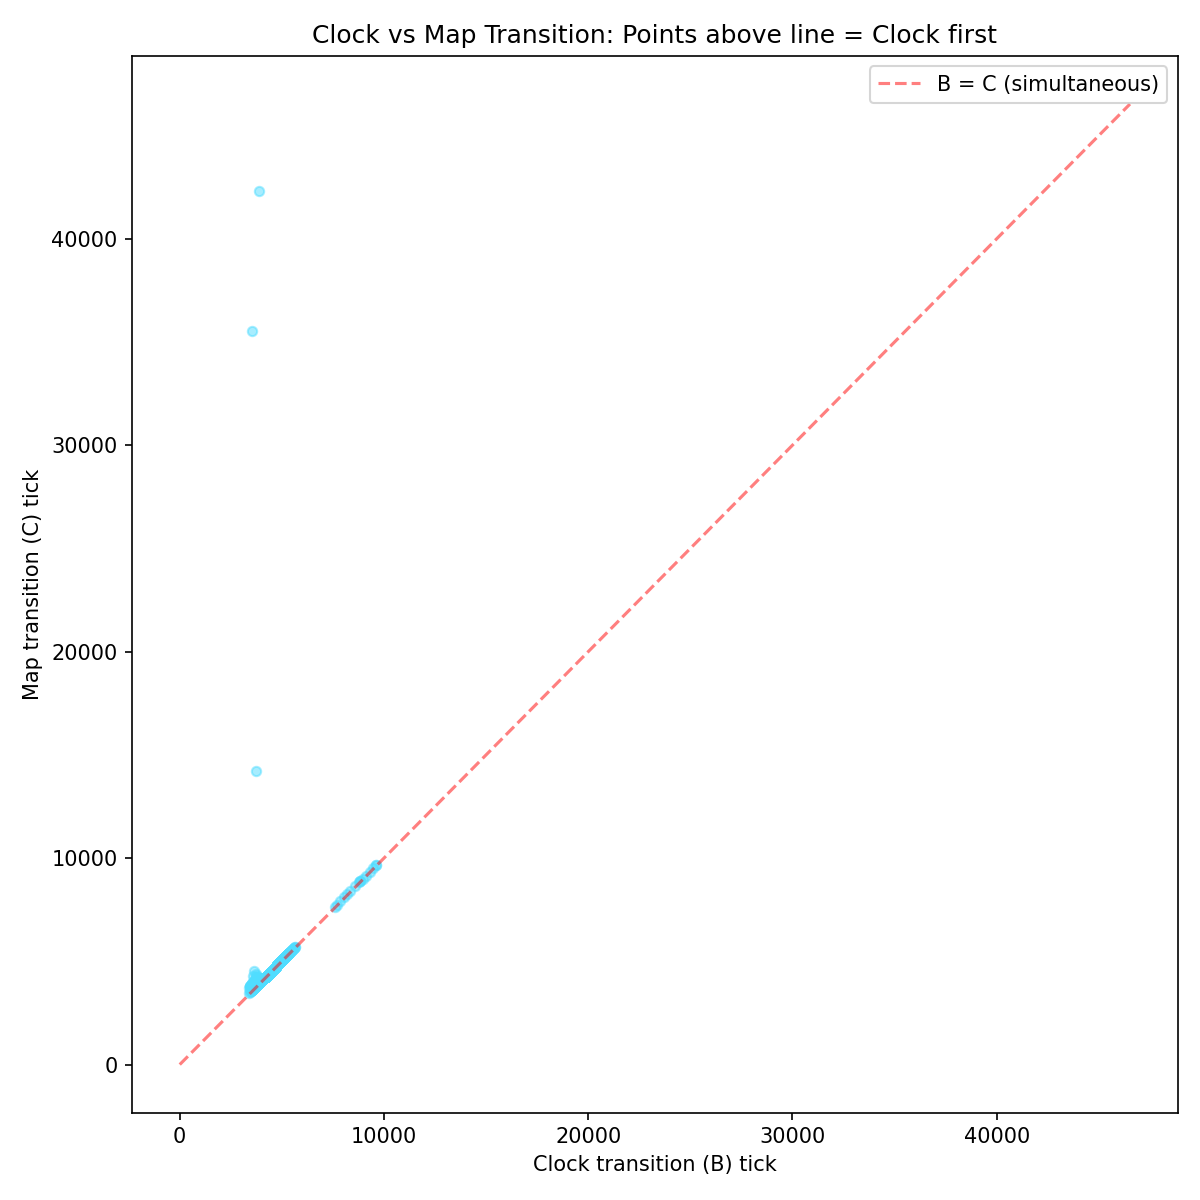
\includegraphics[width=0.75\linewidth]{figures/fig2_clock_vs_map.png}
\caption{\label{fig:scatter}Per-run Clock vs.\ Map transition scatter plot (1D, $N = 482$ runs reaching both phases). Each point represents one simulation. The red dashed diagonal indicates hypothetical simultaneous transition ($B = C$). Every single point lies above the diagonal, indicating the Clock transition occurred before the Map transition in every run without exception.}
\end{figure}

\begin{figure}[H]
\centering
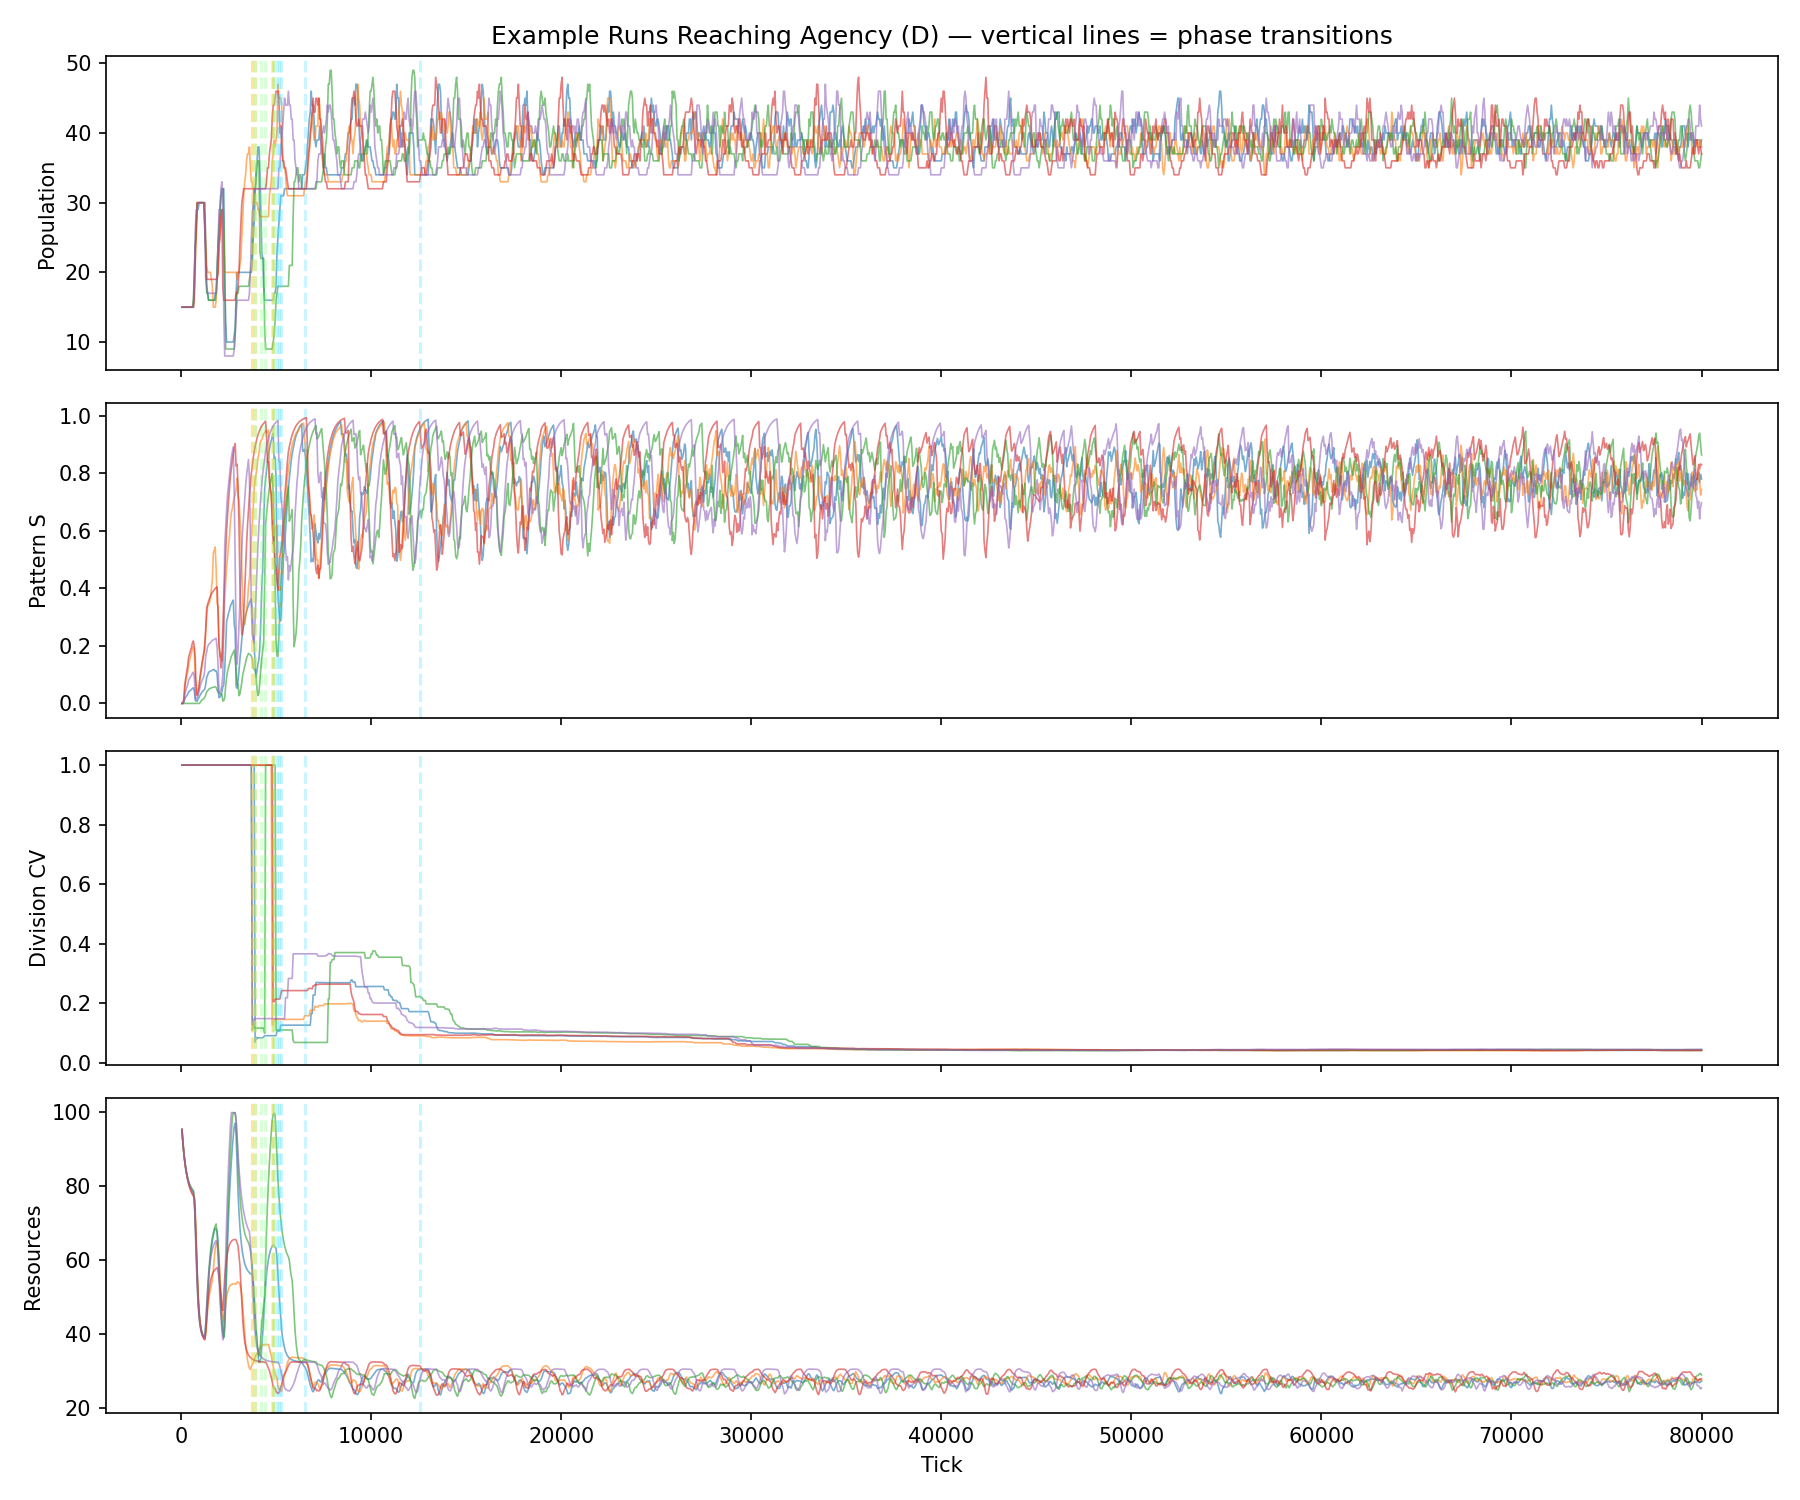
\includegraphics[width=0.95\linewidth]{figures/fig3_example_timeseries.png}
\caption{\label{fig:timeseries}Example time series traces from five runs reaching Phase D. Four panels show population, pattern stability $S$, division CV, and resource levels across 80{,}000 ticks. Vertical dashed lines mark phase transitions (amber = B, green = C, cyan = D). The visual signature of the mandatory ordering is clear: CV crashes first, then $S$ rises, then population stabilizes.}
\end{figure}

\begin{figure}[H]
\centering
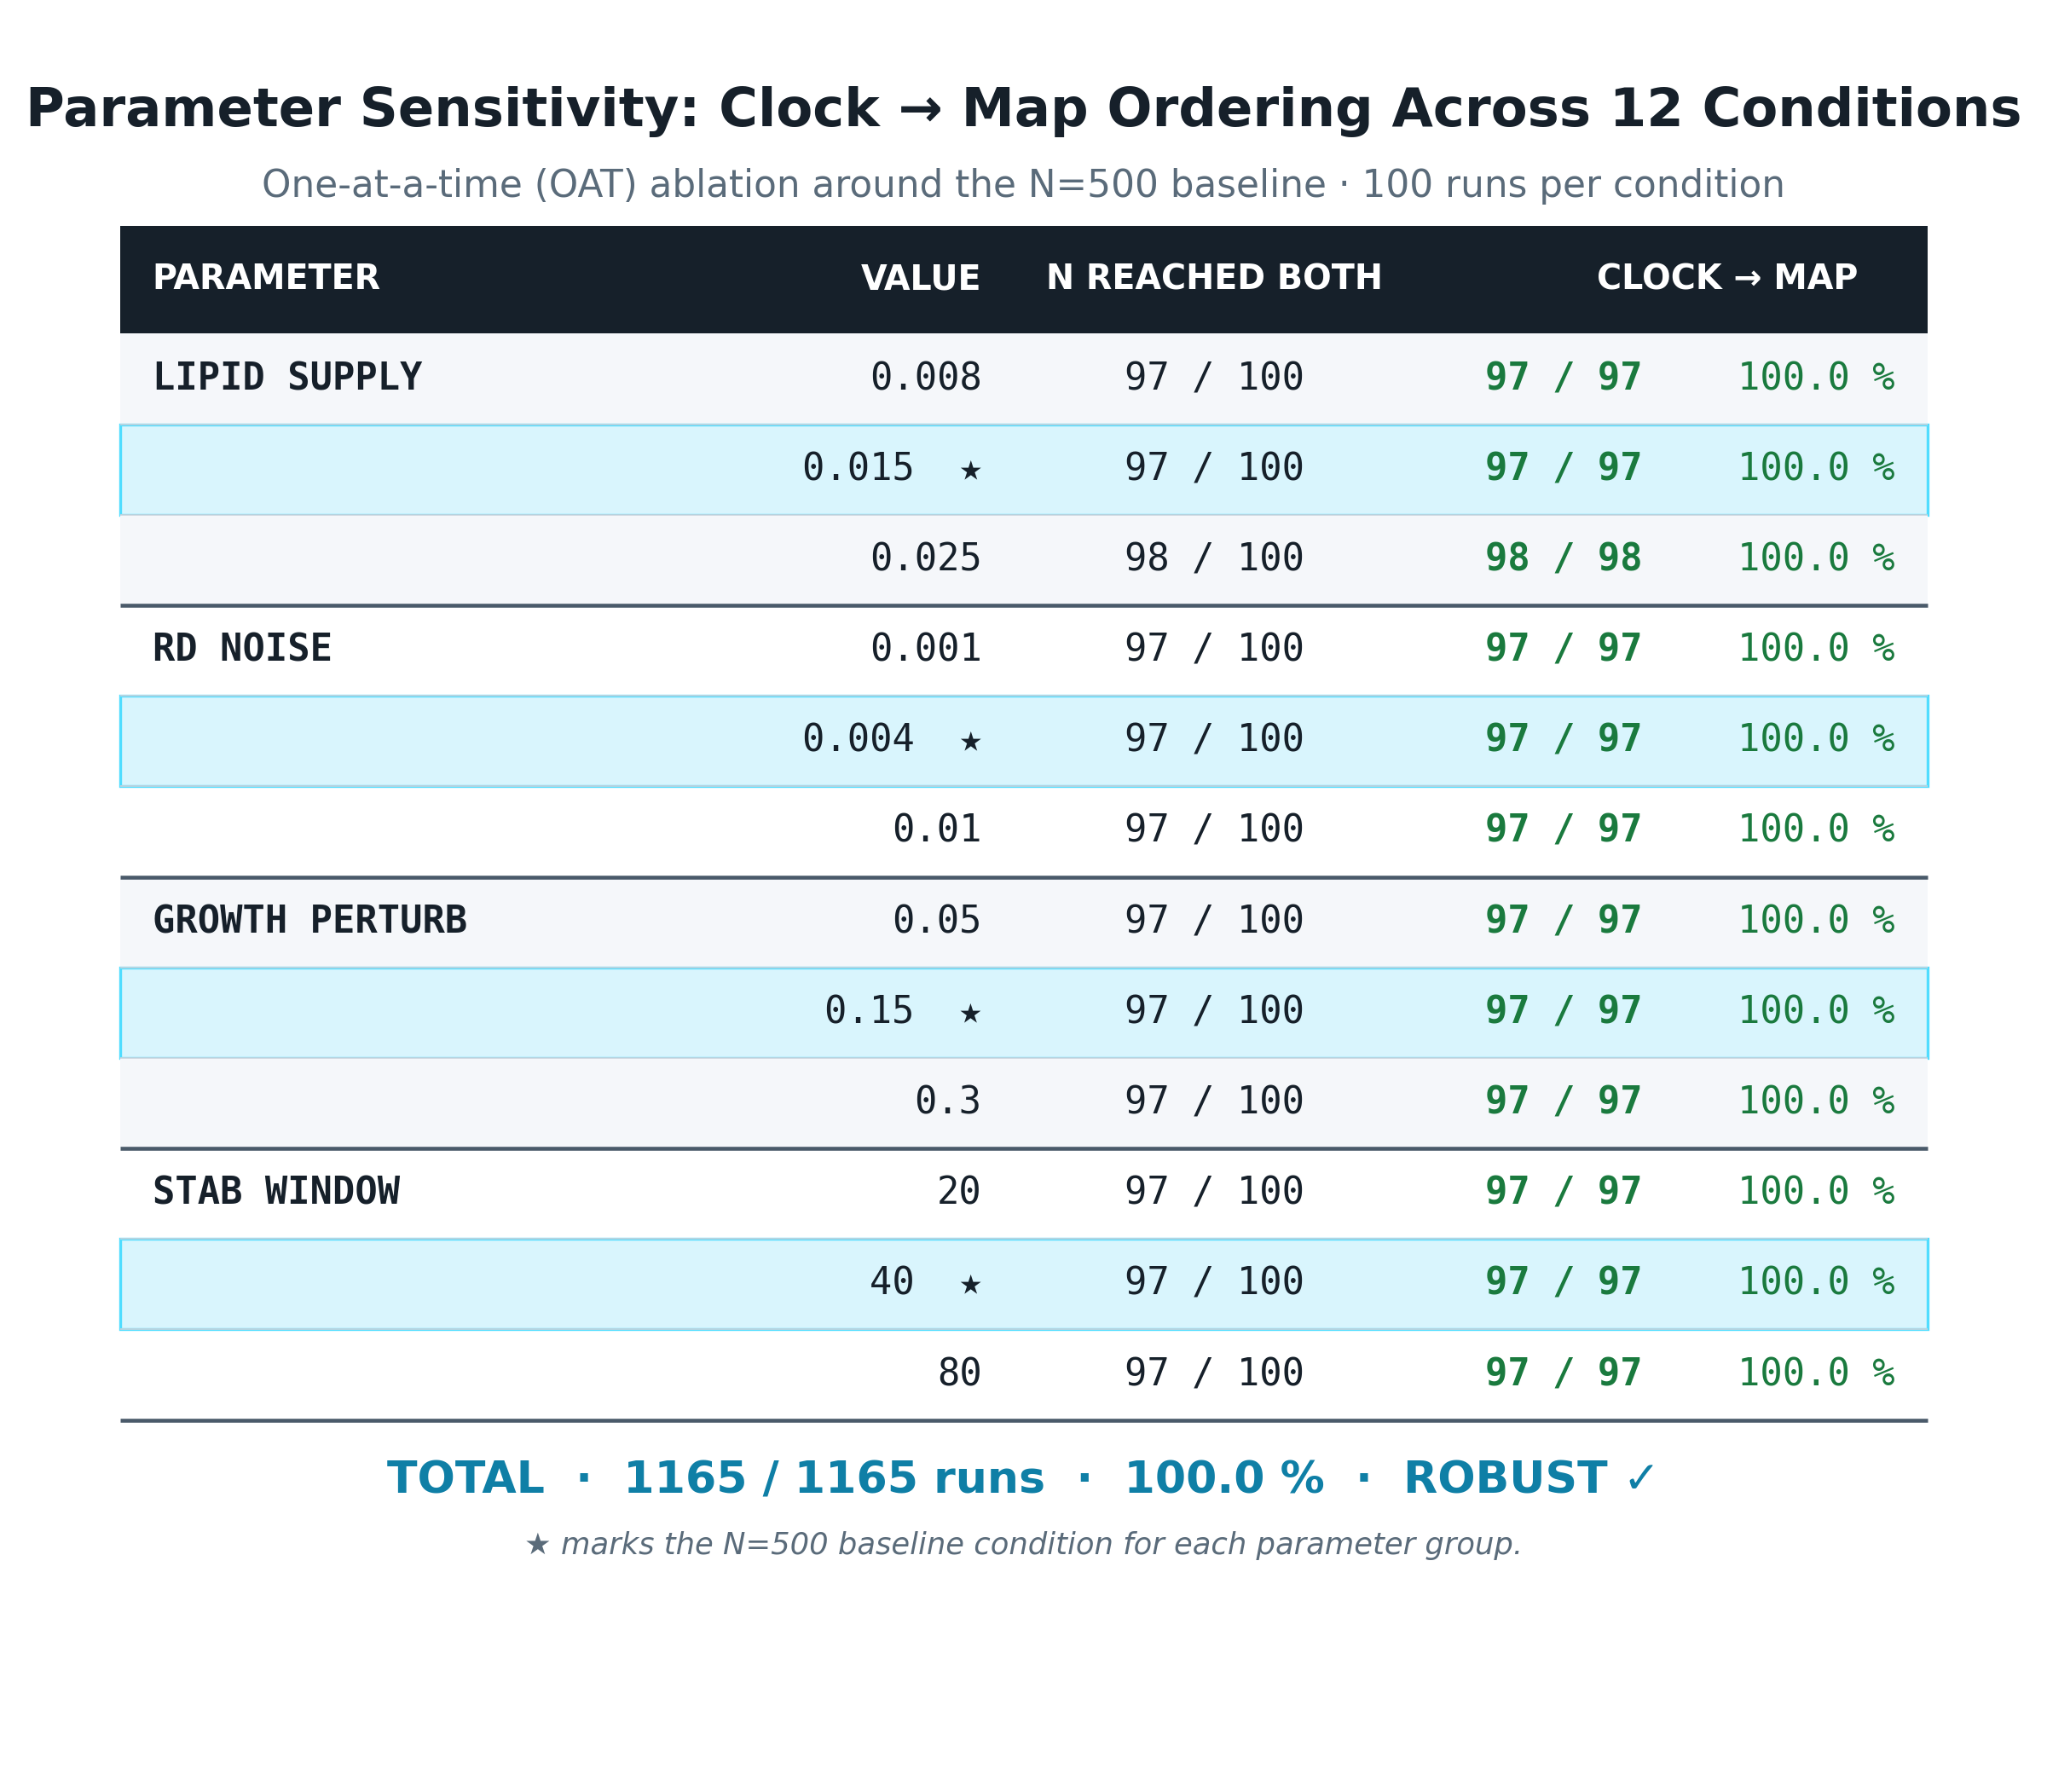
\includegraphics[width=0.85\linewidth]{figures/fig4_ablation_table.png}
\caption{\label{fig:ablation}Parameter sensitivity ablation results table. Twelve conditions across four parameters at three values each. Every cell shows 100\% Clock-before-Map ordering, confirming robustness.}
\end{figure}

\begin{figure}[H]
\centering
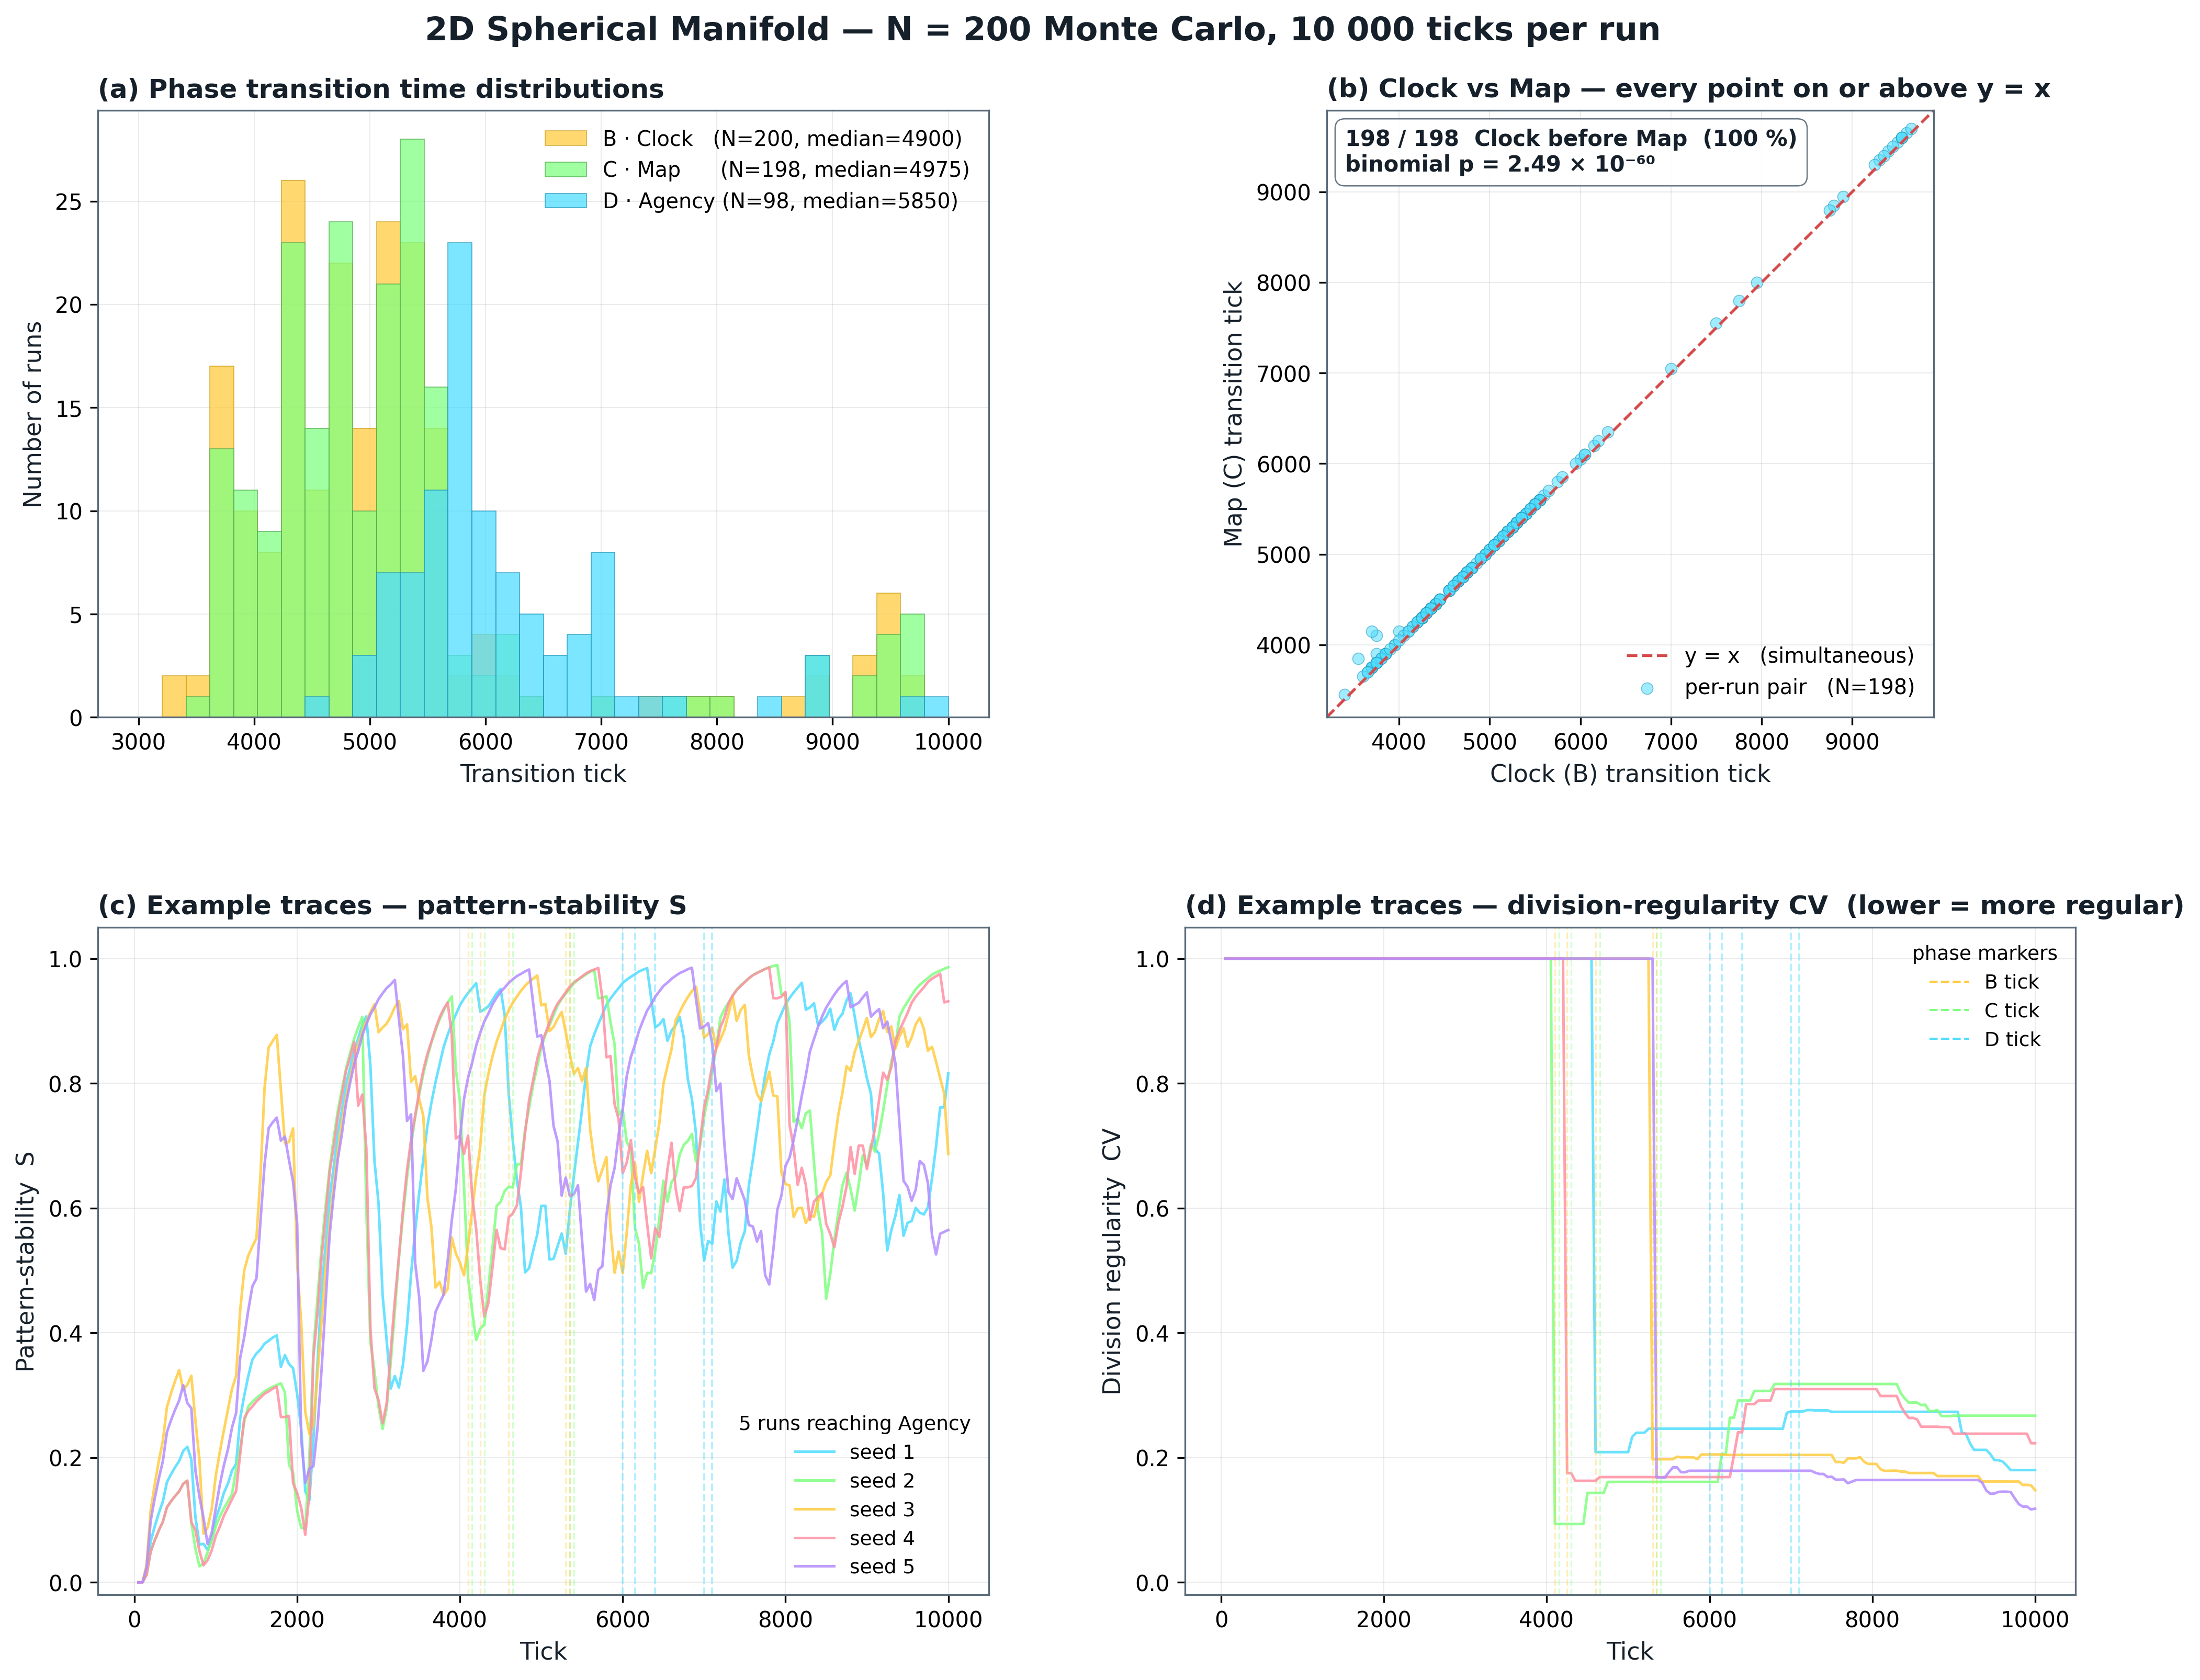
\includegraphics[width=0.95\linewidth]{figures/fig5_2d_sphere_results.png}
\caption{\label{fig:sphere}2D spherical manifold Monte Carlo results ($N = 200$). Four-panel layout: (a) phase transition histograms showing the same temporal ordering as 1D; (b) Clock-vs-Map scatter with every point above diagonal; (c) icosphere rendering showing a representative organized protocell with visible pattern complexity; (d) example time series traces with phase markers.}
\end{figure}

\begin{figure}[H]
\centering
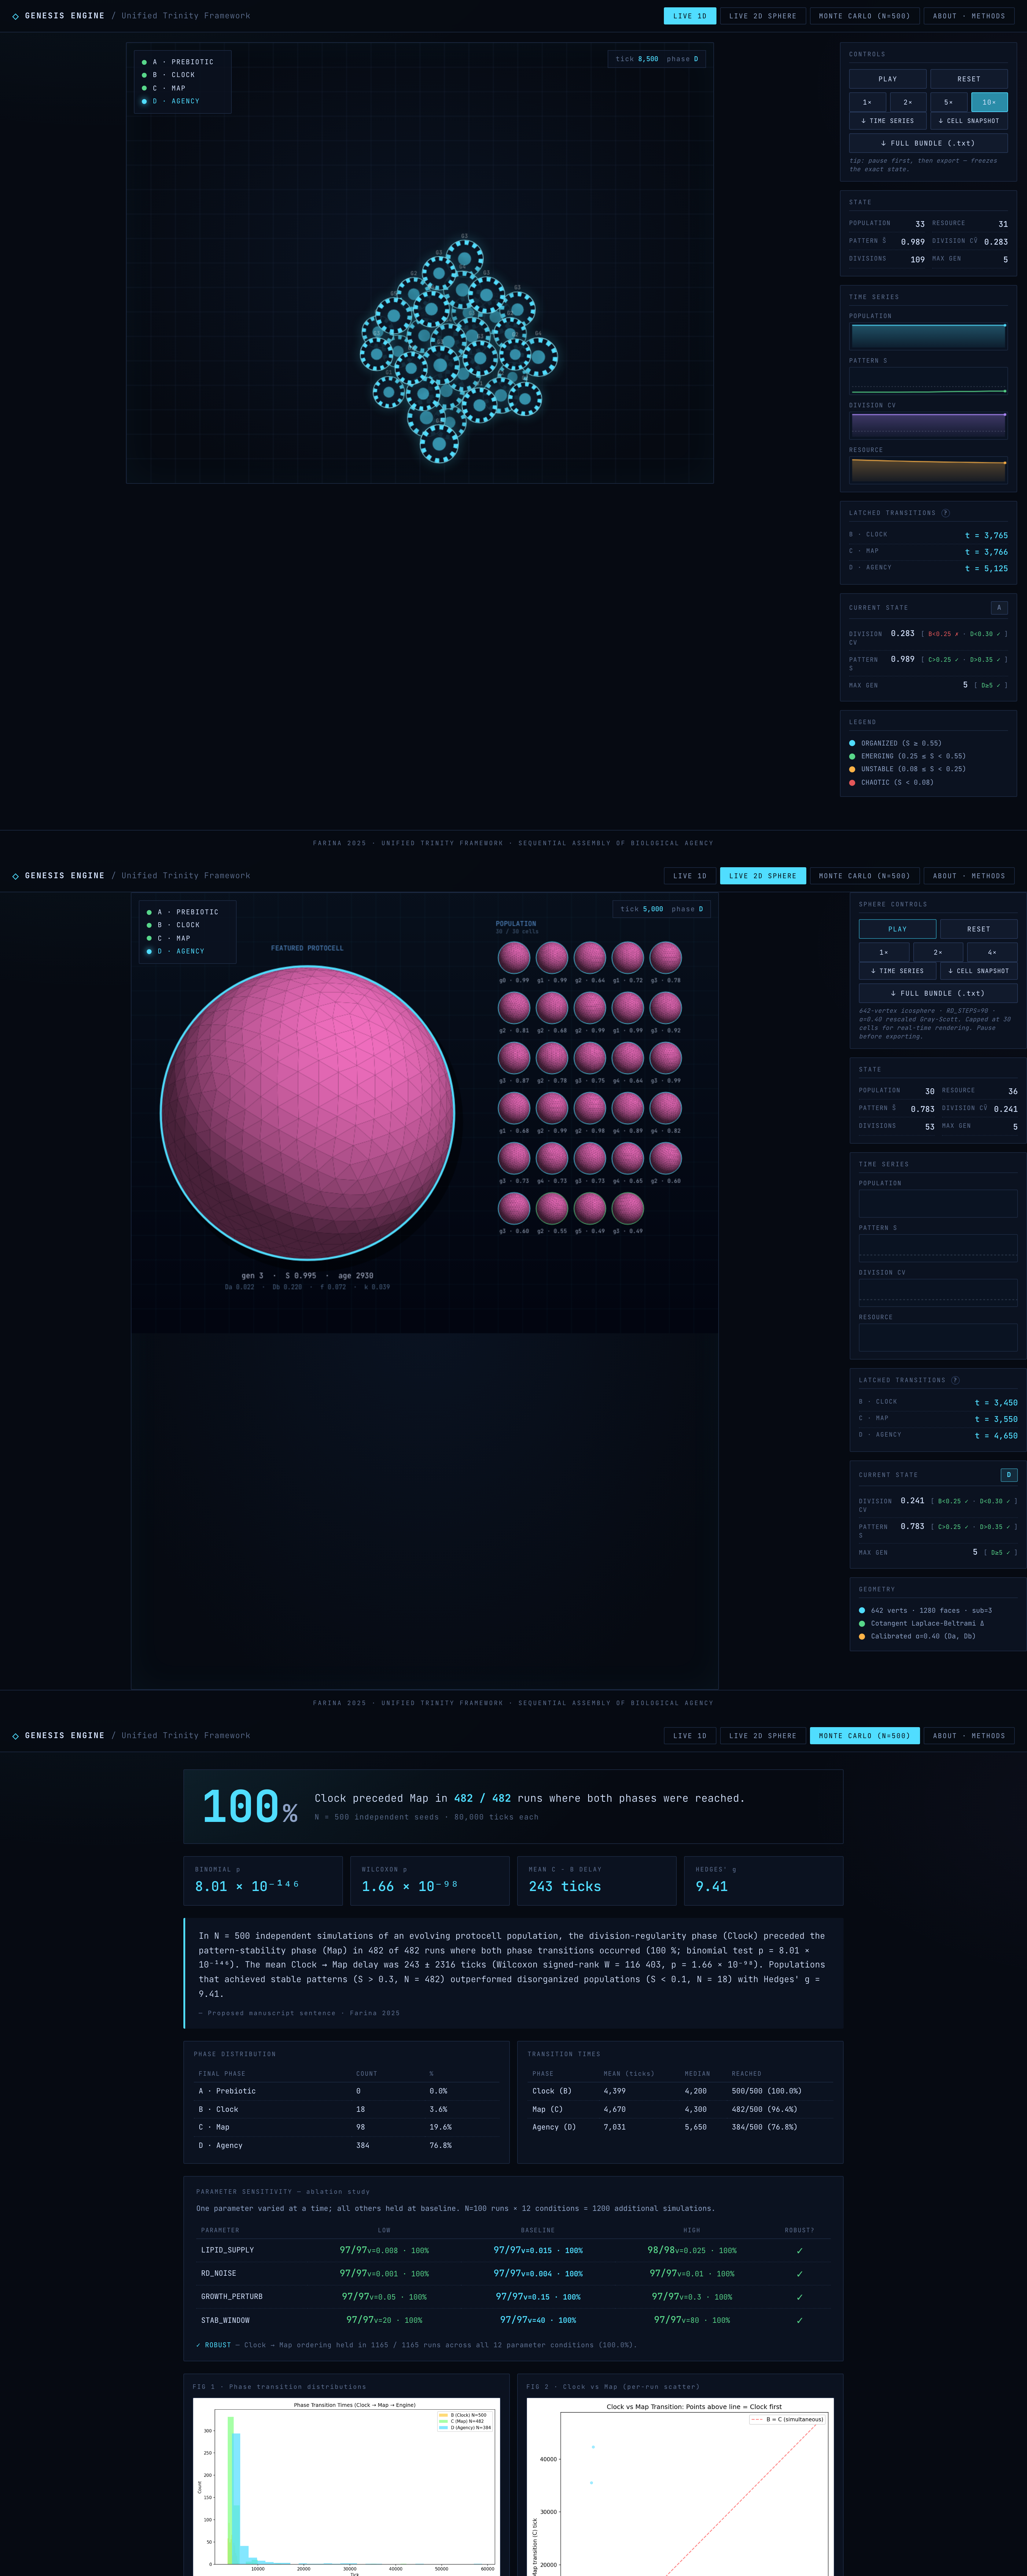
\includegraphics[width=0.95\linewidth]{figures/fig6_dashboard_vertical.png}
\caption{\label{fig:dashboard}Interactive dashboard screenshots (three-panel vertical composite). Top: Live 1D simulation in Phase D, showing organized cyan protocell population with all four phase transitions marked. Middle: Live 2D sphere simulation showing featured protocell with magenta pattern on icosphere surface and population grid. Bottom: Monte Carlo results tab showing the 100\% headline, key statistics, phase distribution table, and ablation sensitivity table. The split \textsc{Latched Transitions} / \textsc{Current State} display provides honest distinction between latched phase events (the statistical measure) and current predicate status (which may drift).}
\end{figure}

\begin{figure}[H]
\centering
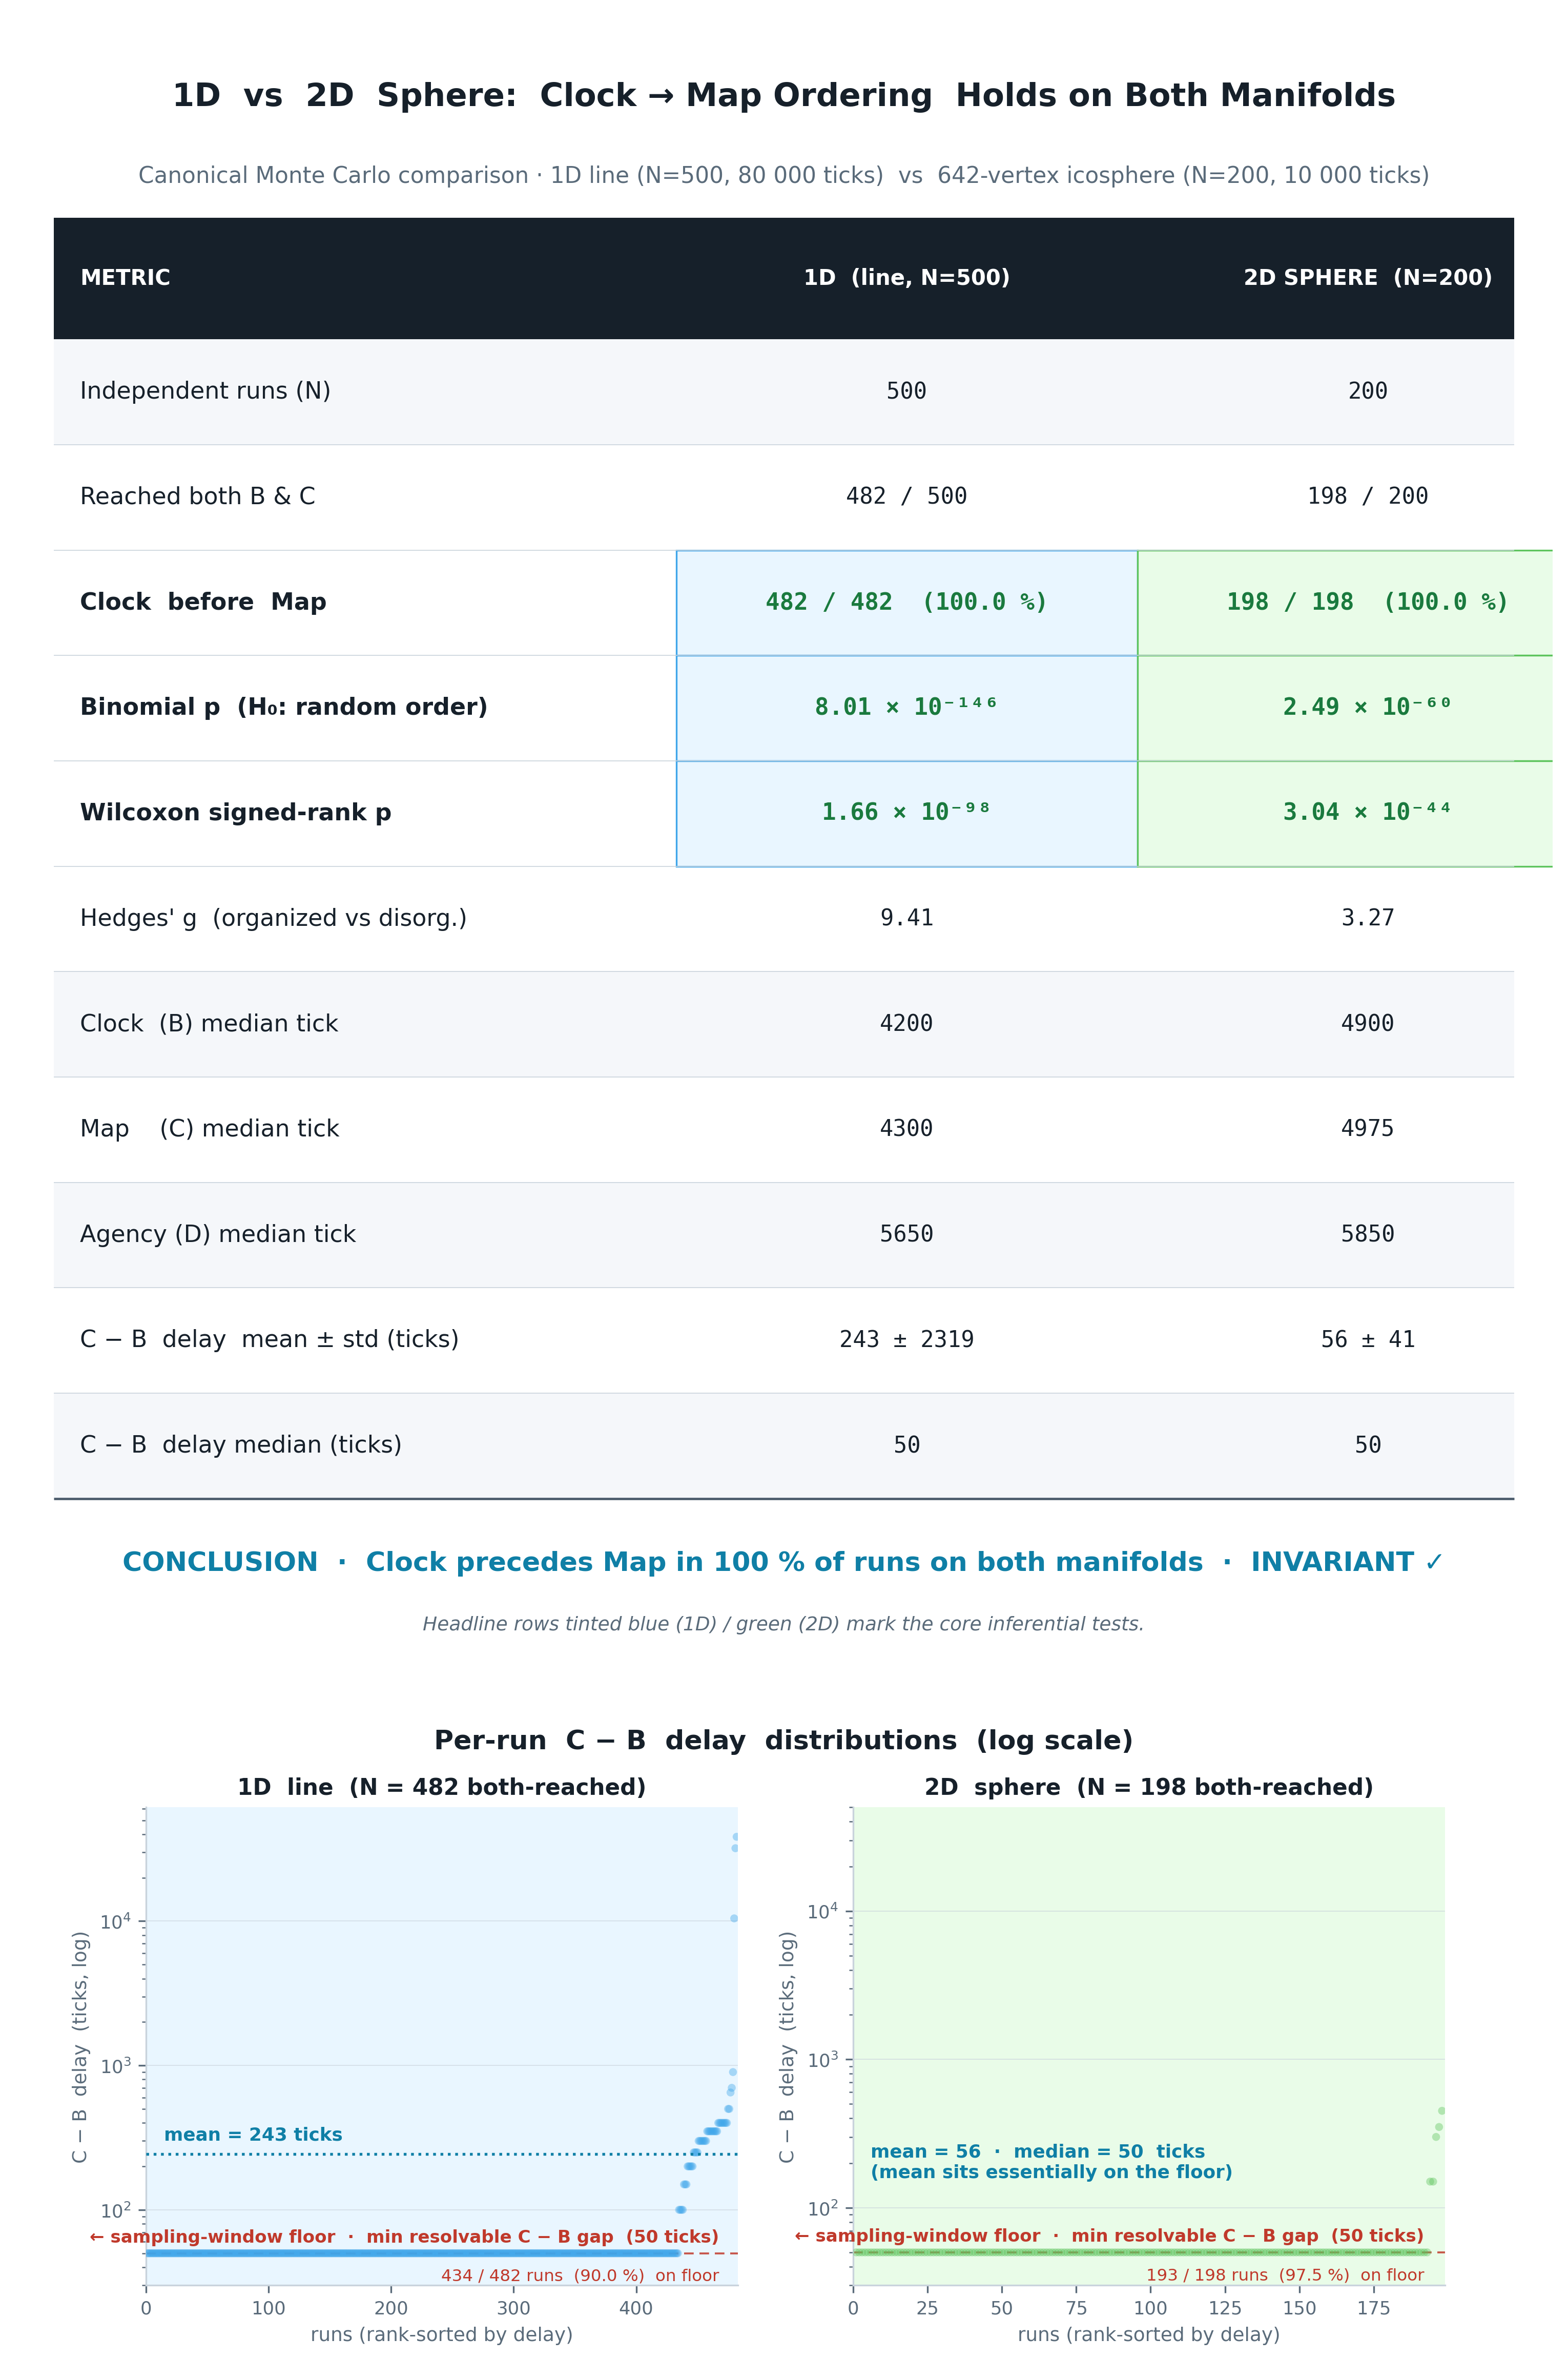
\includegraphics[width=0.82\linewidth]{figures/fig7_comparison_1d_2d.png}
\caption{\label{fig:comparison}Side-by-side comparison of 1D and 2D results. Key metrics: Clock-before-Map ratio (identical 100\%), binomial $p$-value, Wilcoxon $p$-value, Hedges' $g$ effect size, and mean delay. A horizontal reference line at 50 ticks marks the sampling-window floor (minimum resolvable $C-B$ gap given our 50-tick measurement interval). The 1D mean delay of 243 ticks sits well above this floor, providing the strongest evidence that the Clock-to-Map gap is a real physical separation rather than a measurement artifact. The 2D mean of 56 ticks approaches the sampling floor but remains strictly positive across all 198 runs.}
\end{figure}

\end{document}
